\documentclass[a4 paper]{article}
% Set target color model to RGB
\usepackage[inner=1.5cm,outer=1.5cm,top=2.5cm,bottom=2.5cm]{geometry}
\usepackage{setspace}
\usepackage[rgb]{xcolor}
\usepackage{verbatim}
\usepackage{amsgen,amsmath,amstext,amsbsy,amsopn,tikz,amssymb,tkz-linknodes}
\usepackage{fancyhdr}
\usepackage[colorlinks=true, urlcolor=blue,  linkcolor=blue, citecolor=blue]{hyperref}
\usepackage[colorinlistoftodos]{todonotes}
\usepackage{rotating}
%\usetikzlibrary{through,backgrounds}
\hypersetup{%
pdfauthor={Arman Shokrollahi},%
pdftitle={Homework},%
pdfkeywords={Tikz,latex,bootstrap,uncertaintes},%
pdfcreator={PDFLaTeX},%
pdfproducer={PDFLaTeX},%
}
%\usetikzlibrary{shadows}
\usepackage[francais]{babel}
\usepackage{booktabs}
\newcommand{\ra}[1]{\renewcommand{\arraystretch}{#1}}

      \newtheorem{thm}{Theorem}[section]
      \newtheorem{prop}[thm]{Proposition}
      \newtheorem{lem}[thm]{Lemma}
      \newtheorem{cor}[thm]{Corollary}
      \newtheorem{defn}[thm]{Definition}
      \newtheorem{rem}[thm]{Remark}
      \numberwithin{equation}{section}

\newcommand{\homework}[6]{
   \pagestyle{myheadings}
   \thispagestyle{plain}
   \newpage
   \setcounter{page}{1}
   \noindent
   \begin{center}
   \framebox{
      \vbox{\vspace{2mm}
    \hbox to 6.28in { {\bf\hfill} }
       \vspace{6mm}
       \hbox to 6.28in { {\Large \hfill #1 (#2)  \hfill} }
       \vspace{6mm}
       \hbox to 6.28in { {\it Instructor: #3 \hfill Student: #5} }
       %\hbox to 6.28in { {\it TA: #4  \hfill #6}}
      \vspace{2mm}}
   }
   \end{center}
   \markboth{#5 -- #1}{#5 -- #1}
   \vspace*{4mm}
}

\newcommand{\bbF}{\mathbb{F}}
\newcommand{\bbX}{\mathbb{X}}
\newcommand{\bI}{\mathbf{I}}
\newcommand{\bX}{\mathbf{X}}
\newcommand{\bY}{\mathbf{Y}}
\newcommand{\bepsilon}{\boldsymbol{\epsilon}}
\newcommand{\balpha}{\boldsymbol{\alpha}}
\newcommand{\bbeta}{\boldsymbol{\beta}}
\newcommand{\0}{\mathbf{0}}

\begin{document}
\homework{Actividad \#7}{Espacio Fase}{Carlos Liz\'arraga Celaya}{}{Antonio Cota Rodr\'iguez}{}

\section*{Introducci\'on}
\setlength{\parindent}{1.2em}

Hemos estudiado en las pr\'acticas anteriores cual es el comportamiento de un p\'endulo simple y hemos resuelto la ecuaci\'on diferencial tanto para el caso de \'angulos pequeños como para amplitudes arbitrarias. Ahora nos toca gr\'aficar el espacio fase generado por el p\'endulo dadas las condiciones iniciales. Primero definiremos que es el espacio fase.

\subsection*{Espacio Fase}
En mec\'anica cl\'asica, el espacio f\'asico, espacio de fases o diagrama de fases es una construcci\'on matem\'atica que permite representar el conjunto de posiciones y momentos conjugados de un sistema de part\'iculas. Más t\'ecnicamente, el espacio de fases es una variedad diferenciable de dimensi\'on par, tal que las coordenadas de cada punto representan tanto las posiciones generalizadas como sus momentos conjugados correspondientes. Es decir, cada punto del espacio f\'asico representa un estado del sistema f\'isico. Ese estado f\'isico vendr\'a caracterizado por la posici\'on de cada una de las part\'iculas y sus respectivos momentos.  

\begin{figure}[!ht]
  \centering
      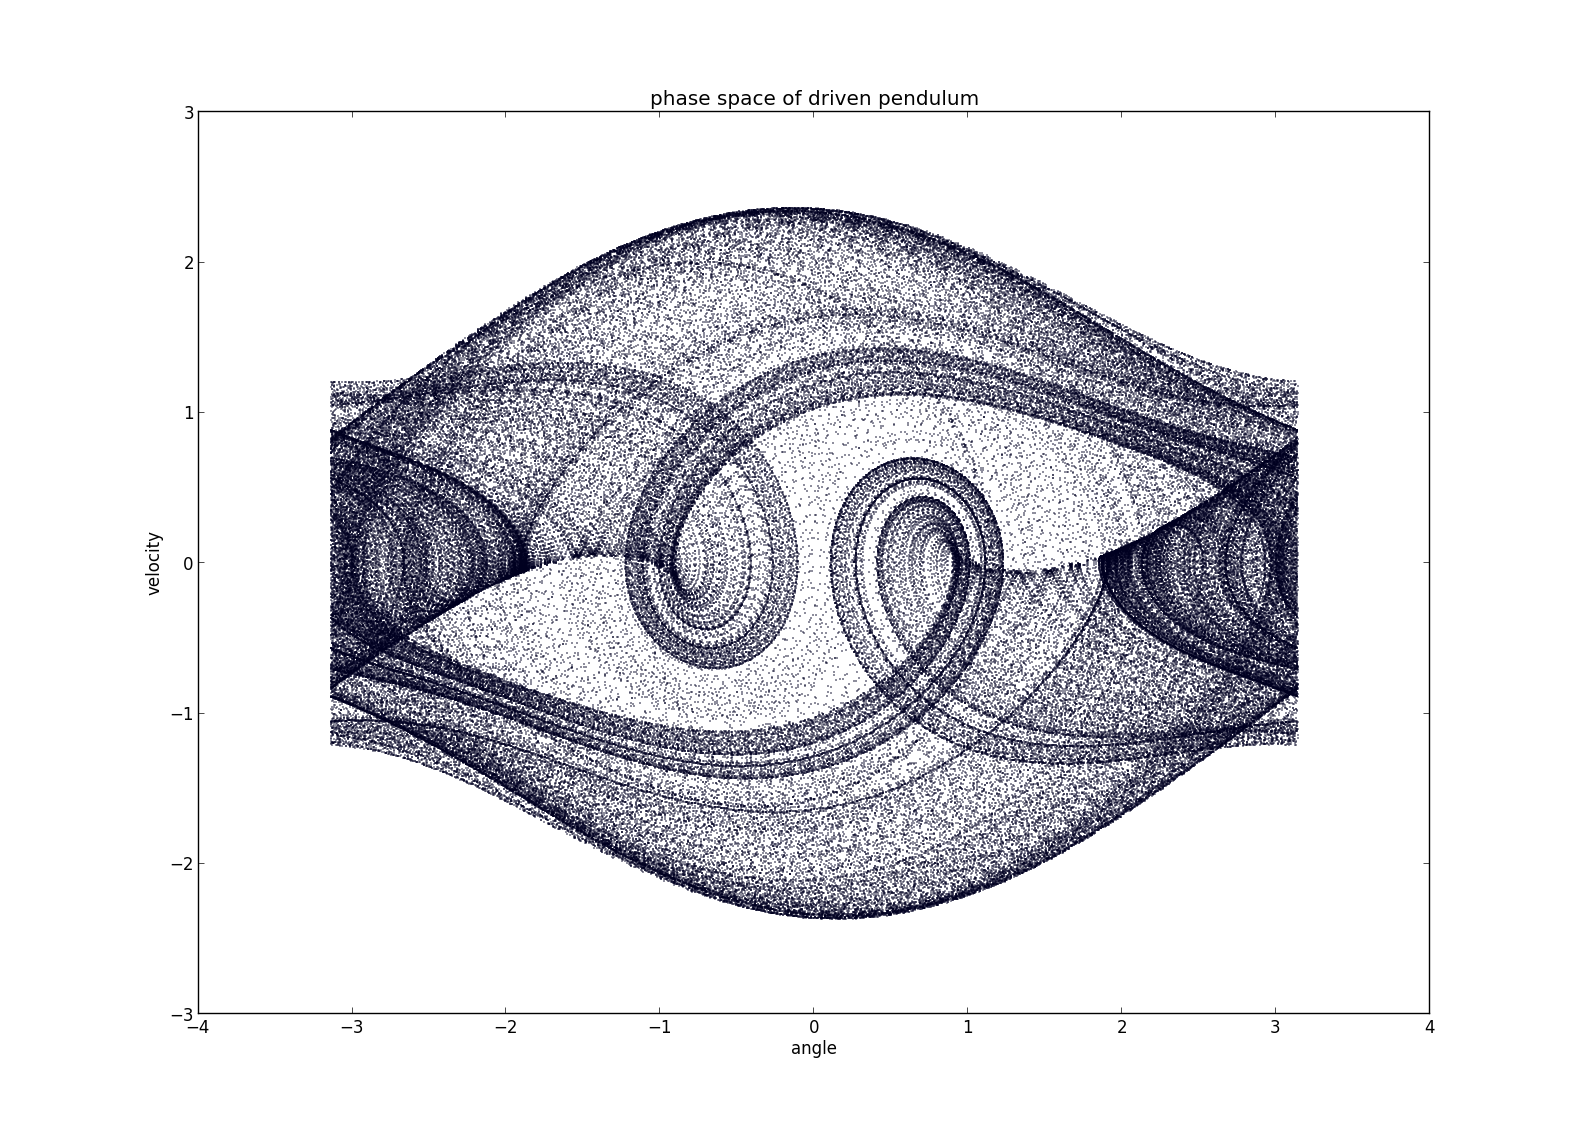
\includegraphics[width=9cm, height=6cm]{PenduloForzado.png}
  \caption{Espacio fase de un p\'endulo forzado (ejemplo)}
\end{figure}

\section*{Programa}

En el siguiente programa resolver\'a la ecuaci\'on diferencial del p\'endulo utilizando el m\'etodo {\bf scipy.integrate.odeint}

\begin{verbatim}
import numpy as np
from scipy.integrate import odeint
import matplotlib.pyplot as plt
import pylab as p

# Utilzaremos las siguientes contantes
g = 9.8
l = 3.0
b = 0.0 
c = g/l

# Condiciones iniciales
X_f1 = np.array([-5.0*np.pi,3.0*np.pi])
X_f2 = np.array([-4.0*np.pi,-0.0*np.pi]) 
t = np.linspace(0,4.0*np.pi,1000) 

# Ecuacion diferencial
def p (y, t, u, v):
    theta, omega = y
    dy_dt = [omega,-u*omega -v*np.sin(theta)]
    return dy_dt

# EL estilo

values  = np.linspace(-1,1,120)   
vcolors = plt.cm.PuBu(np.linspace(1.0,1.0, len(values)))
plt.figure(2)

for v, col in zip(values, vcolors):
    y0 = v * X_f1                              
    
    X = odeint(p, y0, t, args=(b,c))         
    plt.plot( X[:,0], X[:,1], lw=3.5*v, color=col, label='X0=(%.f, %.f)' % ( y0[0], y0[1]) )

for v, col in zip(values, vcolors):
    y1 = v * X_f2                           
    X1 = odeint(p, y1, t, args=(b,c))           
    plt.plot( X1[:,0], X1[:,1], lw=3.5*v, color=col, label='X0=(%.f, %.f)' % ( y1[0], y1[1]) )

# Grafica
plt.title('Espacio fase')
plt.xlabel(r'$ \theta $')
plt.ylabel('$\omega$')
plt.grid()
plt.xlim(-2.0*np.pi,2.0*np.pi)
plt.ylim(-7,7)
plt.show()

\end{verbatim}

Con su respectiva gr\'afica:

\begin{figure}[!ht]
  \centering
      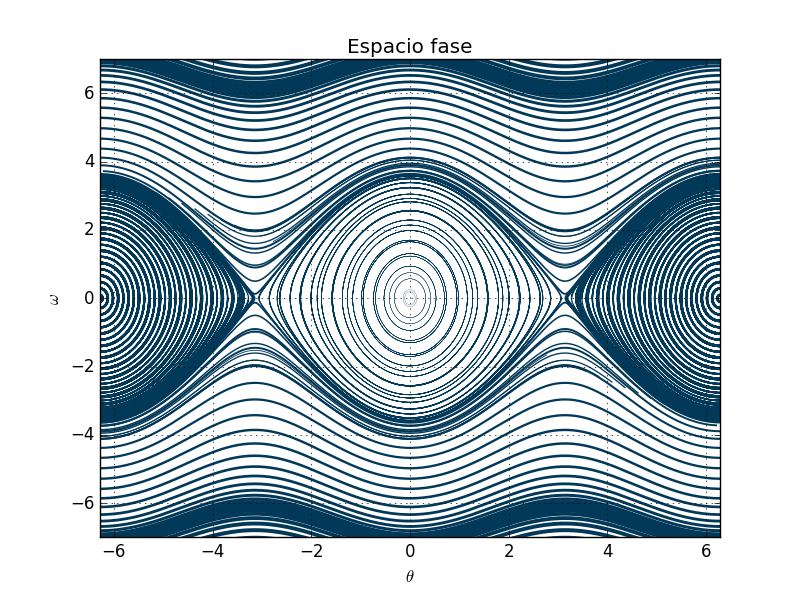
\includegraphics[width=9cm, height=6cm]{EP_Pendulo.png}
  \caption{Espacio fase de nuestro p\'endulo}
\end{figure}


\end{document}